 
\begin{figure}[tbp] 
  \centering
  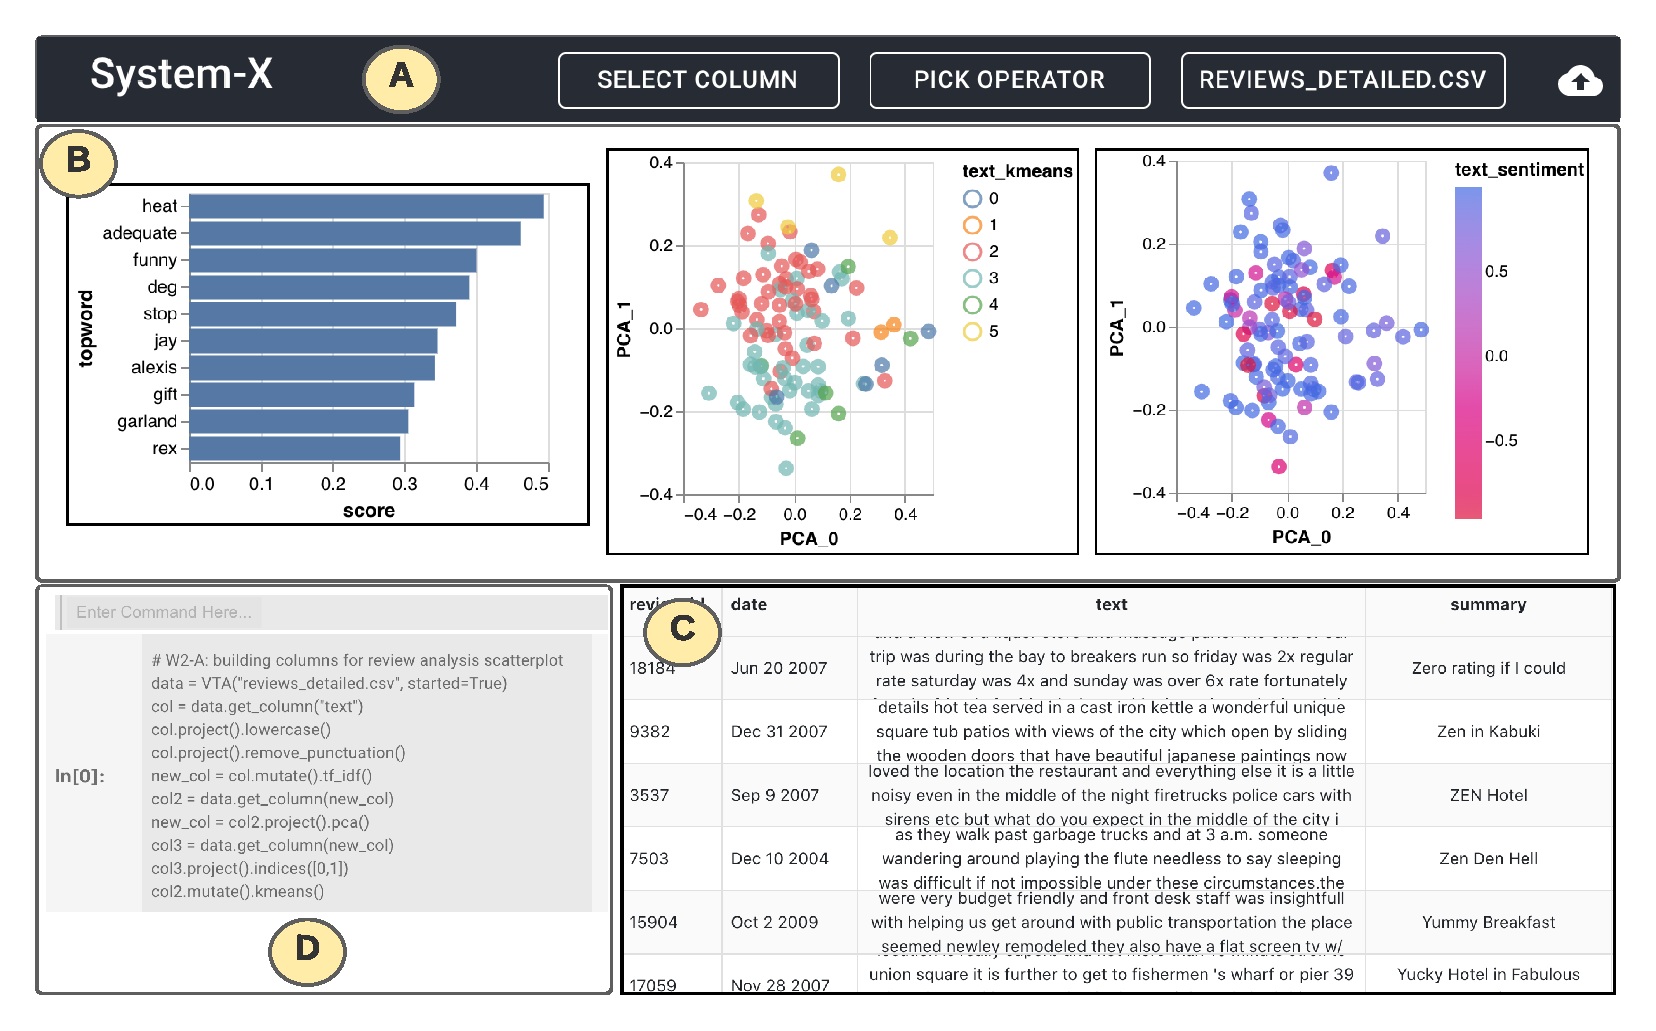
\includegraphics[width=\linewidth]{figures/leam_fe.pdf}
  \caption{\small \system user interface. (A) Operator View enables users to perform visual text analytics (\vita) operations using drop-down menus, (B) Visualization View 
  holds a carousel of interactive visualizations created by users, (C) Table View displays the data and its subsequent transformations, and (D) Notebook View allows users to compose and run \vita operations using a declarative language. Inset (E) shows the \vta JSON specification for the bar chart operator in Operator View. Inset (F) shows a declarative \vta command for interacting with the bar chart from Notebook View. \label{fig:fe}} 
\end{figure}

\section{Introduction}\label{sec:intro}
% motivate the problem space and its relevance and impact 
The internet has become the platform for many of our everyday activities, from shopping to dating. The global market size of e-commerce has exponentially increased in the last decade. 
The upward trend is expected to be continued.  A recent study projects the worldwide e-commerce sales to be around six trillion dollars by 2023~\cite{ecommerce}, nearly a 50\% increase over the current market. This growth has contributed to the proliferation of digital text, particularly user-generated text (reviews, Q\&As, discussions), which often contain useful information for improving the services and products on the web. Enterprises increasingly adopt text mining technologies to extract, analyze, and summarize information from such unstructured text data.

% online text is noisy in many senses, which warrants systems taking integrative 
% approach to their analysis 
However, online text collections are notoriously noisy, incomplete, ambiguous, subjective and often sparse in informational content. Consider reviews; a review about a hotel, for example, typically refers to only a few qualities about the hotel, such as location and service, out of many possible.  Discovering, cleaning, analyzing, searching, modeling, extracting information from, and identifying and exploring topics in such text collections can be daunting and time consuming without integrated systems that take the whole text analytics pipeline 
into account. 

The characteristics of online text make interactive workflows and visualizations not only appealing but also essential for accessible, rapid iterative analysis~\cite{ittoo2016text}.
Therefore we here focus on visual interactive text analysis (\vita hereafter) and related systems. There are a few commercial (e.g.,~\cite{sastextminer,rapidminer,tableau,powerbi}) 
and open-source tools (e.g.,\cite{perez2007ipython,nltk,gensim,spacy}) that can  support different stages of \vita at varying degrees~\cite{liu2018bridging, mlbazaar}. For example, spreadsheets allow directly processing and manipulating  data, computational notebooks enable flexible exploratory analysis and modeling, and visualization systems, typically based on chart templates, facilitate quick interactive visual analysis.  An ideal system would unify these affordances~\cite{kandel2011research,drosos2020wrex,wu2020b2}.  There are also many customized visual text analytics tools~\cite{liu2018bridging}, often in the form of research prototypes, that focus on specific use-cases like review exploration~\cite{zhang2020teddy}, sentiment analysis~\cite{kucher2018state}, and text summarization~\cite{carenini2006interactive}.
Unfortunately, none of these solutions accommodate the inherently cyclic, 
trial-and-error-based nature of \vita pipelines end to end in an integrated manner. 


\todo{Expand and revise to answer the question: Why is it difficult to develop an end-to-end \vita system?} 
\vita is an iterative and non-linear process---it is a multistage process that involves tasks like data preprocessing and transformation, model building, hypothesis testing, and insight exploration, all of which require multiple iterations to obtain satisfactory outcomes. While having end-to-end  \vita systems is much desired, designing and building them is difficult. The primary 
   challenge is the number and diversity of the tasks that need to be supported. In part, 
   programmatic tools such as computational notebooks can provide extensibility and 
   expressivity to incrementally build such support but they often lack in interactivity, 
   accessibility, and scalability, impeding non-linear iterative analysis. 

%  :  (a) extensibility and expressivity of \vita workflows, (b) their continuity and reproducibility, (c) data heterogeneity and provenance, and (d) coordination  of user interactions.  The challenges identified here are informed by our experience in developing data systems, working with practitioners as part of an industry research lab, part of a larger company with more than three hundred e-commerce subsidiaries and prior research, particularly those  reporting from interview studies on data analysis workflows~\cite{zhang2020teddy,lee2020demystifying},

\todo{Revise and complete. BTW, `one-stop-shop' might  offend some reviewers. } 
In response, we propose \system, a one-stop-shop for visual interactive text analysis. \system combines the advantages of spreadsheets, computational notebooks, and visualization tools by integrating a Notebook View with interactive views of raw and transformed data (Figure~\ref{fig:fe}). A key component in the design of \system is a visual text algebra (\vta) that enables users to specify complex \vita operations over heterogeneous data and their visual representations; either using a declarative language in the Notebook View (Figure~\ref{fig:fe}F) or by creating operators in the front-end that translates to \vta specifications (Figure~\ref{fig:fe}E) in JSON (JavaScript Object Notation). Through usage examples, we demonstrate the expressivity of \vta and how it enables \system to support diverse tasks ranging from data cleaning to visualization. Moreover, to facilitate efficient execution of \vta on heterogeneous data, we introduce a new data model extending dataframes called \vitaframe.
To evaluate \system, we conduct two case studies using two popular Kaggle text 
analytics workflows for tweet analysis and spam detection, respectively, and elicit 
user feedback. Our findings suggest \system is $\ldots$. We have made the current 
version of \system open-source at~\url{https://github.com/chi-author/system-x}.
